\documentclass[fleqn]{article}

%%%%%%%%%%%%%%%%%%%%% Pre-document %%%%%%%%%%%%%%%%%%%%%
\usepackage{fancyhdr}
\usepackage{titlesec}
\usepackage{float}
\usepackage{array}
\usepackage{nicematrix}
\usepackage{multicol}
\usepackage{enumitem}
\usepackage{listings}
\usepackage{xcolor}
\usepackage{scrextend}
\usepackage{tikz}

\setlength{\parindent}{0pt} % Remove auto paragraph indents
\renewcommand\labelitemi{{\boldmath$\cdot$}}
\setlength{\mathindent}{0pt}  

% Get rid of those big margins
\usepackage[margin=1in]{geometry}
\newlength\titleindent
\setlength\titleindent{2cm}

\begin{document}

\pagestyle{fancy}
% Header
\fancyhead{}
\fancyhead[L]{Liam Gilligan, Stephanie L'Heureux}
\fancyhead[R]{\thepage}
% No page numbers for footer
\fancyfoot{}

\lstset{language=C++,
    basicstyle=\ttfamily,
    keywordstyle=\color{blue}\ttfamily,
    stringstyle=\color{red}\ttfamily,
    commentstyle=\color{teal}\ttfamily,
    morecomment=[l][\color{magenta}]{\#}
}

\begin{center}
    \Large{\textbf{Arduino Lab 2}}\\
\end{center}
\vspace{0.25in}

\section*{Introduction}
The second and final Arduino lab for CS-24 involved developing a "not a bomb" countdown timer using two 7-segment displays to indicate time set/remaining controlled by a rotary encoder. The user may turn the rotary encoder to incrementally select a value between 0.0 and 9.9 seconds. Pressing the encoder button evokes countdown mode in which the timer decreases by 0.1 second intervals. The countdown continues until it reaches zero or is interrupted by adjustments to the rotary encoder. This report discusses the components used and implementation as well as some challenges faced and solutions.
\section*{Background}
The countdown timer utilizes several hardware components, including two 7-segment displays, two 74HC595 shift registers, and a rotary encoder. The following sections provide an overview of these components and explain the basic principles of their operation.
\subsection*{7-segment display}
A 7-segment display is a component featuring seven LED segments arranged in an "8-shaped" pattern, which may be illuminated in different combinations to display numbers and some letters. Each segment is an independent LED, controlled by a pins (labeled a–g) and connected through either a common cathode or anode. When power is applied to a pin, the corresponding segment lights up.

\begin{table}[H]
    \centering
    \setlength{\tabcolsep}{2pt}
    \fontsize{8pt}{12pt}\selectfont
    \begin{tabular}{cccccccccc}
    \begin{tikzpicture}[line width=2.5pt, scale=0.75]
    \draw[red] (0.1, 2) -- (0.9, 2) node[midway, above, red] {\small a};
    \draw[red] (1,1.9) -- (1,1.1) node[midway, right, red] {\small b};
    \draw[red] (1,0.9) -- (1,0.1) node[midway, right, red] {\small c};
    \draw[red] (0.9,0) -- (0.1,0) node[midway, below, red] {\small d};
    \draw[red] (0,0.1) -- (0,0.9) node[midway, left, red] {\small e};
    \draw[red] (0,1.1) -- (0,1.9) node[midway, left, red] {\small f};
    \draw[lightgray] (0.1,1) -- (0.9,1) node[midway, below, lightgray] {\small g};
    \end{tikzpicture}  
    & 
    \begin{tikzpicture}[line width=2.5pt, scale=0.75]
    \draw[lightgray] (0.1, 2) -- (0.9, 2) node[midway, above, lightgray] {\small a};
    \draw[red] (1,1.9) -- (1,1.1) node[midway, right, red] {\small b};
    \draw[red] (1,0.9) -- (1,0.1) node[midway, right, red] {\small c};
    \draw[lightgray] (0.9,0) -- (0.1,0) node[midway, below, lightgray] {\small d};
    \draw[lightgray] (0,0.1) -- (0,0.9) node[midway, left, lightgray] {\small e};
    \draw[lightgray] (0,1.1) -- (0,1.9) node[midway, left, lightgray] {\small f};
    \draw[lightgray] (0.1,1) -- (0.9,1) node[midway, below, lightgray] {\small g};
    \end{tikzpicture} 
    &
    \begin{tikzpicture}[line width=2.5pt, scale=0.75]
    \draw[red] (0.1, 2) -- (0.9, 2) node[midway, above, red] {\small a};
    \draw[red] (1,1.9) -- (1,1.1) node[midway, right, red] {\small b};
    \draw[lightgray] (1,0.9) -- (1,0.1) node[midway, right, lightgray] {\small c};
    \draw[red] (0.9,0) -- (0.1,0) node[midway, below, red] {\small d};
    \draw[red] (0,0.1) -- (0,0.9) node[midway, left, red] {\small e};
    \draw[lightgray] (0,1.1) -- (0,1.9) node[midway, left, lightgray] {\small f};
    \draw[red] (0.1,1) -- (0.9,1) node[midway, below, red] {\small g};
    \end{tikzpicture} 
    &  
    \begin{tikzpicture}[line width=2.5pt, scale=0.75]
    \draw[red] (0.1, 2) -- (0.9, 2) node[midway, above, red] {\small a};
    \draw[red] (1,1.9) -- (1,1.1) node[midway, right, red] {\small b};
    \draw[red] (1,0.9) -- (1,0.1) node[midway, right, red] {\small c};
    \draw[red] (0.9,0) -- (0.1,0) node[midway, below, red] {\small d};
    \draw[lightgray] (0,0.1) -- (0,0.9) node[midway, left, lightgray] {\small e};
    \draw[lightgray] (0,1.1) -- (0,1.9) node[midway, left, lightgray] {\small f};
    \draw[red] (0.1,1) -- (0.9,1) node[midway, below, red] {\small g};
    \end{tikzpicture} 
    & 
    \begin{tikzpicture}[line width=2.5pt, scale=0.75]
    \draw[lightgray] (0.1, 2) -- (0.9, 2) node[midway, above, lightgray] {\small a};
    \draw[red] (1,1.9) -- (1,1.1) node[midway, right, red] {\small b};
    \draw[red] (1,0.9) -- (1,0.1) node[midway, right, red] {\small c};
    \draw[lightgray] (0.9,0) -- (0.1,0) node[midway, below, lightgray] {\small d};
    \draw[lightgray] (0,0.1) -- (0,0.9) node[midway, left, lightgray] {\small e};
    \draw[red] (0,1.1) -- (0,1.9) node[midway, left, red] {\small f};
    \draw[red] (0.1,1) -- (0.9,1) node[midway, below, red] {\small g};
    \end{tikzpicture} 
    &
    \begin{tikzpicture}[line width=2.5pt, scale=0.75]
    \draw[red] (0.1, 2) -- (0.9, 2) node[midway, above, red] {\small a};
    \draw[lightgray] (1,1.9) -- (1,1.1) node[midway, right, lightgray] {\small b};
    \draw[red] (1,0.9) -- (1,0.1) node[midway, right, red] {\small c};
    \draw[red] (0.9,0) -- (0.1,0) node[midway, below, red] {\small d};
    \draw[lightgray] (0,0.1) -- (0,0.9) node[midway, left, lightgray] {\small e};
    \draw[red] (0,1.1) -- (0,1.9) node[midway, left, red] {\small f};
    \draw[red] (0.1,1) -- (0.9,1) node[midway, below, red] {\small g};
    \end{tikzpicture} 
    &
    \begin{tikzpicture}[line width=2.5pt, scale=0.75]
    \draw[red] (0.1, 2) -- (0.9, 2) node[midway, above, red] {\small a};
    \draw[lightgray] (1,1.9) -- (1,1.1) node[midway, right, lightgray] {\small b};
    \draw[red] (1,0.9) -- (1,0.1) node[midway, right, red] {\small c};
    \draw[red] (0.9,0) -- (0.1,0) node[midway, below, red] {\small d};
    \draw[red] (0,0.1) -- (0,0.9) node[midway, left, red] {\small e};
    \draw[red] (0,1.1) -- (0,1.9) node[midway, left, red] {\small f};
    \draw[red] (0.1,1) -- (0.9,1) node[midway, below, red] {\small g};
    \end{tikzpicture} 
    & 
    \begin{tikzpicture}[line width=2.5pt, scale=0.75]
    \draw[red] (0.1, 2) -- (0.9, 2) node[midway, above, red] {\small a};
    \draw[red] (1,1.9) -- (1,1.1) node[midway, right, red] {\small b};
    \draw[red] (1,0.9) -- (1,0.1) node[midway, right, red] {\small c};
    \draw[lightgray] (0.9,0) -- (0.1,0) node[midway, below, lightgray] {\small d};
    \draw[lightgray] (0,0.1) -- (0,0.9) node[midway, left, lightgray] {\small e};
    \draw[lightgray] (0,1.1) -- (0,1.9) node[midway, left, lightgray] {\small f};
    \draw[lightgray] (0.1,1) -- (0.9,1) node[midway, below, lightgray] {\small g};
    \end{tikzpicture} 
    &
    \begin{tikzpicture}[line width=2.5pt, scale=0.75]
    \draw[red] (0.1, 2) -- (0.9, 2) node[midway, above, red] {\small a};
    \draw[red] (1,1.9) -- (1,1.1) node[midway, right, red] {\small b};
    \draw[red] (1,0.9) -- (1,0.1) node[midway, right, red] {\small c};
    \draw[red] (0.9,0) -- (0.1,0) node[midway, below, red] {\small d};
    \draw[red] (0,0.1) -- (0,0.9) node[midway, left, red] {\small e};
    \draw[red] (0,1.1) -- (0,1.9) node[midway, left, red] {\small f};
    \draw[red] (0.1,1) -- (0.9,1) node[midway, below, red] {\small g};
    \end{tikzpicture} 
    &
    \begin{tikzpicture}[line width=2.5pt, scale=0.75]
    \draw[red] (0.1, 2) -- (0.9, 2) node[midway, above, red] {\small a};
    \draw[red] (1,1.9) -- (1,1.1) node[midway, right, red] {\small b};
    \draw[red] (1,0.9) -- (1,0.1) node[midway, right, red] {\small c};
    \draw[lightgray] (0.9,0) -- (0.1,0) node[midway, below, lightgray] {\small d};
    \draw[lightgray] (0,0.1) -- (0,0.9) node[midway, left, lightgray] {\small e};
    \draw[red] (0,1.1) -- (0,1.9) node[midway, left, red] {\small f};
    \draw[red] (0.1,1) -- (0.9,1) node[midway, below, red] {\small g};
    \end{tikzpicture} 
    \end{tabular}
    \caption{Segments illuminated to display numbers 0-9}
    \label{table1}
\end{table}

\subsection*{Shift register}
The 74HC595 shift register is used to reduce the number of GPIO pins required to control devices. It converts 8-bits of input read over serial (\verb|DS|) to eight parallel data outputs (\verb|Q0| through \verb|Q7|). The built-in Arduino \verb|shiftout()| function may be used to send 8-bits to the shift register, given the \verb|DS| pin, clock pin (\verb|ST|), the order to shift the bits out (\verb|MSBFIRST| or \verb|LSBFIRST|), and the data to output.

\subsection*{Rotary encoder}
An incremental rotary encoder is a device that detects changes in rotational movement. Rotation is detected by the sensor by generating two square waves output to the A and B channel, or pins \verb|CLK| and \verb|DT| respectively. When the knob is rotated, the square waves are adjusted. If rotated clockwise, the \verb|CLK| pin is \verb|LOW|, followed subsequently by a \verb|LOW| signal on the \verb|DT| pin. Counterclockwise motion produces the opposite results. Both pins quickly return to the \verb|HIGH| state. By analyzing the offsets square waves, the direction of rotation is determined. 


\section*{Implementation}
This section outlines the implementation of the countdown timer, detailing some fundamental decisions in both hardware and software.

\subsection*{Hardware}
\subsubsection*{Reducing GPIO pins required}
Two 7-segment displays show either the time remaining or the time set by the user, depending on the timer's state. If the displays were directly connected to the Arduino, a 7-segment display would require 8 GPIO pins, resulting in a total of 16 pins to control both displays. However, by using a shift register, the design is streamlined. The shift register accepts an 8-bit serial input and converts it to eight parallel outputs, which control the eight LED pins of the 7-segment display. Using two 74HC595 shift registers, the hardware and software simplifies significantly. In terms of software, now a single binary string representation may sent to the shift register rather than of managing each segment independently (more information below). Furthermore, and most importantly, this method reduces the number of GPIO pins needed to control the two displays to just 6, a 62.5\% reduction in the number of pins needed.

\subsubsection*{General implementation}
Hardware was created and tested in Wokwi, a browser-based microcontroller simulator. All components were organized on a breadboard for easy connections and usage of common ground and 5V rails. Colored, neatly organized wires were also used to keep track of the connections.

\subsection*{Software}
\subsubsection*{Program states}
The countdown timer has two basic states, "rotation mode" in which the user selects a start time with the rotary encoder and "countdown mode" where the timer counts down in increments of 0.1s. The software is structured in a way in which it checks what state it is in, and executes the expected behavior of that state unless an interruption condition is encountered, in which the state is changed. This approach simplifies the behavior into two discrete functionaries which must be achieved.

\subsubsection*{Read and track rotations}
The \verb|check_rot_rotation()| function reads channel A and channel B from the rotary encoder and determines the rotation. The function returns is 1 if rotated clockwise, -1 if rotated counter clockwise, 0 if not rotated. The result is passed to \verb|increment_max_time()| which adds the rotation to a global \verb|max_time| counter, ensuring the \verb|max_time| does not exceed 99 or fall below 0.

\subsubsection*{Display time}
In a section above, the general principals of a 7-segment display were discussed. If we note that power on is a 1 and power off is 0, each configuration to display a digit may be simplified to a 8-bit binary representation of the form \verb|abcdefgDP| (Table 2). Making use of the shift register as mentioned in the previous section, 0-9 may then may be simplified to binary strings. These can be stored in an array \verb|int_to_seg| for simple conversion from decimal to 7-segment binary representation.

\vspace*{0.15cm}
To display the \verb|max_time| on the 7-segment displays, first the first and second digit are isolated. These values are used as an index into the \verb|int_to_seg| array, converting the base 10 integer into a 8-bit representation for the 7-bit display. The number from the tens place is or-ed with 1 to evoke the DP (decimal point) bit. These values are then sent to the shift registers using \verb|shiftout()|

\subsubsection*{Countdown mode}
"Countdown mode" is evoked by pressing the button on the rotary encoder. At this time, the user selected \verb|max_time| is decremented by 1, the new \verb|max_time| is displayed and the program delays for 0.1s. This is repeated until the \verb|max_time| reaches 0 or the user turns the rotary encoder. For implementation of checking for rotation during delay, see the following section. 

% \begin{table}[H]
%     \centering
%     \setlength{\tabcolsep}{15pt}
%     \begin{tabular}{cccccccc|c}
%     \textbf{a} & \textbf{b} & \textbf{c} & \textbf{d} & \textbf{e} & \textbf{f} & \textbf{g} & \textbf{DP} & \textbf{digit} \\ \hline
%     1 & 1 & 1 & 1 & 1 & 1 & 0 & x & 0 \\ \hline
%     0 & 1 & 1 & 0 & 0 & 0 & 0 & x & 1 \\ \hline
%     1 & 1 & 0 & 1 & 1 & 0 & 1 & x & 2 \\ \hline
%     1 & 1 & 1 & 1 & 0 & 0 & 1 & x & 3 \\ \hline
%     0 & 1 & 1 & 0 & 0 & 1 & 1 & x & 4 \\ \hline
%     1 & 0 & 1 & 1 & 0 & 1 & 1 & x & 5 \\ \hline
%     1 & 0 & 1 & 1 & 1 & 1 & 1 & x & 6 \\ \hline
%     1 & 1 & 1 & 0 & 0 & 0 & 0 & x & 7 \\ \hline
%     1 & 1 & 1 & 1 & 1 & 1 & 1 & x & 8 \\ \hline
%     1 & 1 & 1 & 0 & 0 & 1 & 1 & x & 9 \\
%     \end{tabular}
%     \caption{Truth table to display digits 0-9}
% \end{table}



\section*{Challenges and solutions}
The most notable challenge encountered was when working with the \verb|delay()| function. This built-in Arduino function stops the entire program execution for a specified duration. In this program, \verb|delay()| is used to wait 0.1s to update the displays. However, during "countdown mode", if the rotary encoder is rotated, the program should exit countdown mode and switch to "rotation mode". This is an issue because the rotary encoder needs to be monitored continuously for changes, but \verb|delay()| halts all program activity. As a result, the encoder is only checked every 0.1s in "countdown mode", making it unable to detect rotations reliably. 

\vspace{0.15cm}
To resolve this, the \verb|delay_and_check_for_rotation()| function was implemented. This function accepts a delay time then loops that many times, checking for rotation and delaying for 1ms each iteration. When the loop is complete, the program will have stopped (about) the requested time, while still checking for rotation at an acceptable interval.

\section*{Conclusion}
The lab was successfully completed and met the specifications in the lab guidelines. 
    \begin{figure}[H]
        \centering
        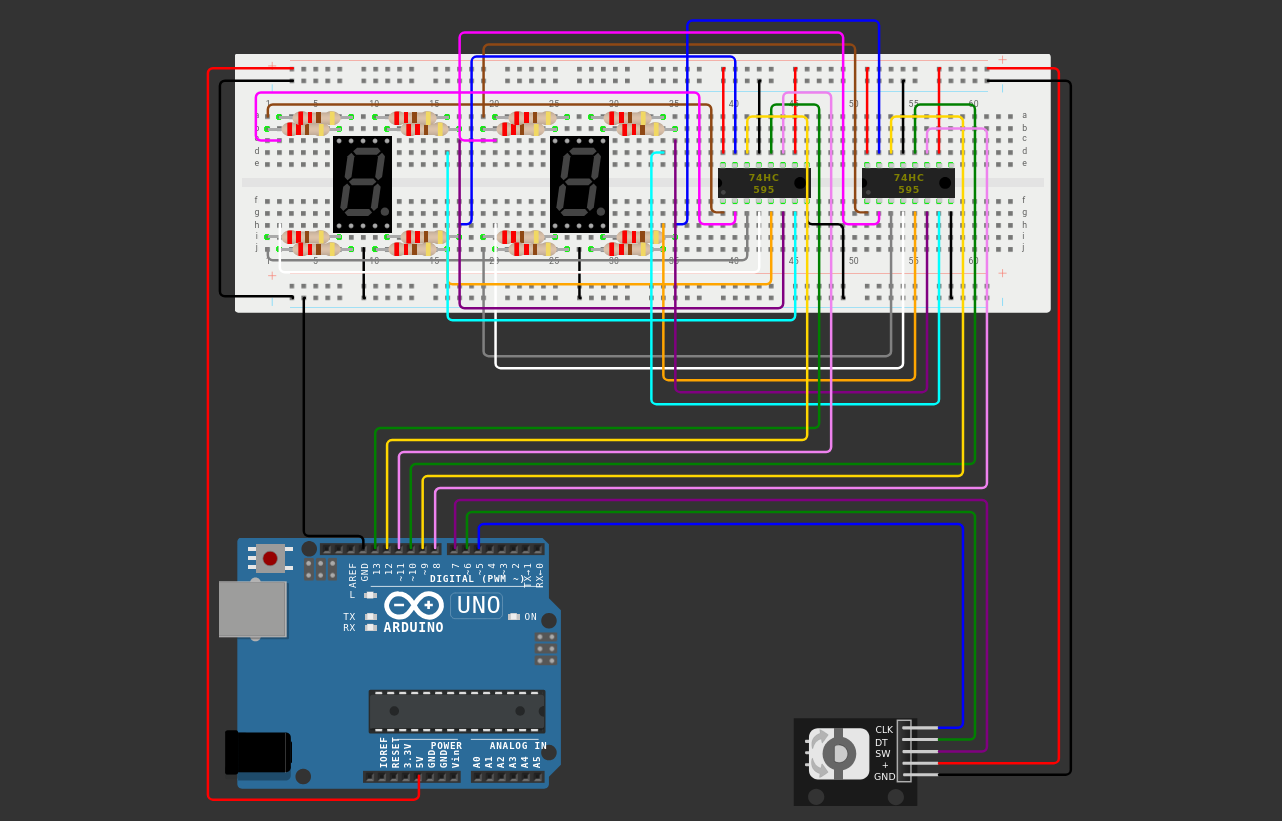
\includegraphics[width=5in]{circut.png}
        \caption{Completed countdown timer hardware.}
    \end{figure}
\end{document}
